\documentclass{article}
\usepackage{fullpage}
\usepackage{float}
\usepackage{graphicx}
\setkeys{Gin}{width=\textwidth,keepaspectratio}%,draft}

\begin{document}

\title{Reference Guide for Stack Tracing Java}
\author{}
\date{2025-05-12}

\maketitle

\section*{FYI}
\begin{itemize}
	\item Only a single color is required for memory diagrams, different colors
	are used (and order written into code) for greater clarity in this document
\end{itemize}

\section{Basic Java}

\begin{verbatim}
	public static void main(String[] args) {
	    int anInt = 10;
	    double aDouble = 5.8;
	    boolean Boolean = true;
	    String aString = "6.3";
	    anInt = 20;
	}
\end{verbatim}

\begin{itemize}
	\item variable changes result in previous values being crossed out and
	new ones written in so that progression can be seen
\end{itemize}

\begin{figure}[H]
	\centering
	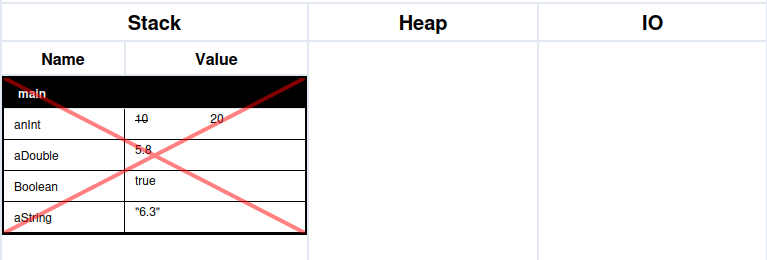
\includegraphics{basicVariables.png}
\end{figure}

\pagebreak


\section{Function calls}

\subsection{Return value}

\begin{verbatim}
	public static double multiplyByTwo(double input) {
	    double x = input * 2;
	    return x;
	}

	public static void main (String[] args) {
	    double x = 7.0;
	    double result = multiplyByTwo(x);
	    result = multiplyByTwo(result);
	    System.out.println(result);
	    int y = 3;
	}
\end{verbatim}

\begin{itemize}
	\item each function call is put in its own stack frame
	\item variables created after the function call appear further down the stack
	\item IO stands for input/output and is where any command line user input or
	outputs in terms of print statements appear
\end{itemize}

\begin{figure}[H]
	\centering
	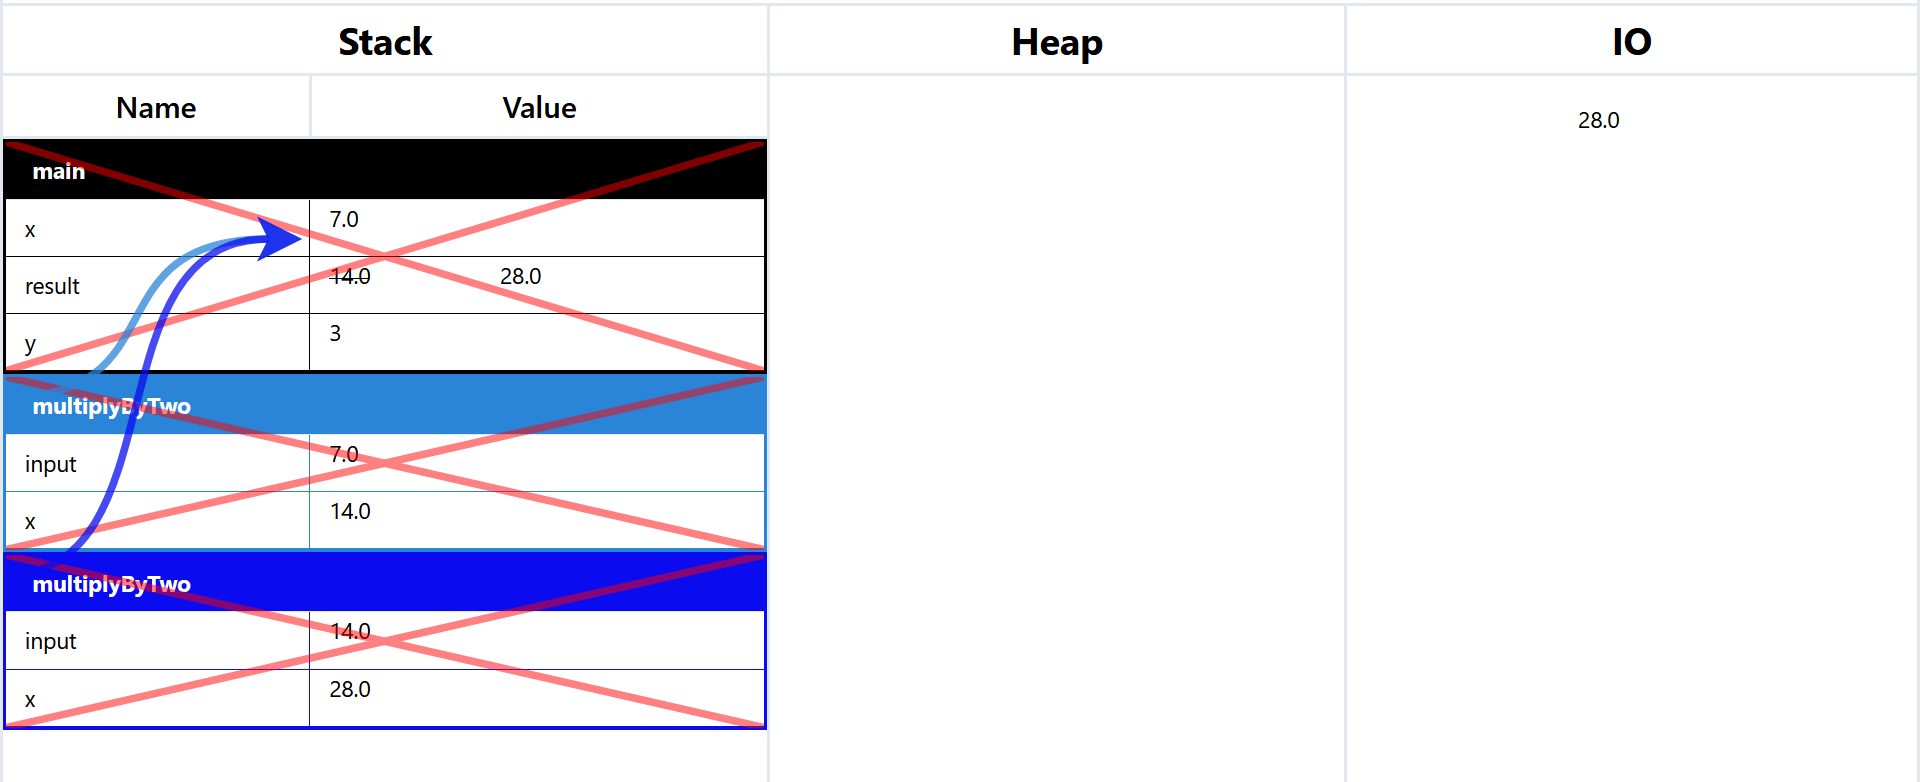
\includegraphics{functionReturn.png}
\end{figure}

\pagebreak

\subsection{No return value}

\begin{verbatim}
	public static double printValue(int a) {
	    int temp = n+2;
	    System.out.println("temp == " + temp);
	}

	public static void main (String[] args) {
	    printValue(4);
	}
\end{verbatim}

\begin{figure}[H]
	\centering
	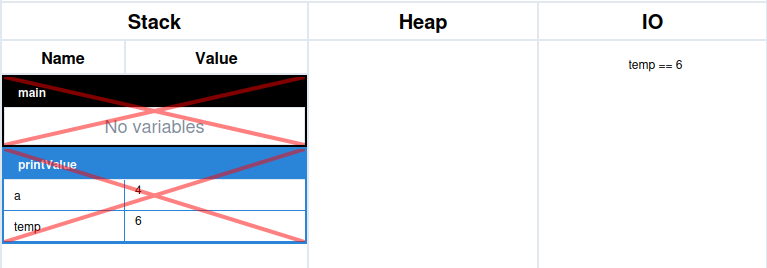
\includegraphics{functionNoReturn.png}
\end{figure}

\pagebreak

\section{For loops}

\subsection{Basic}

\begin{verbatim}
	public static void main (String[] args) {
	    int x = 4;
	    for (int i = 1; i < 5; i++) {
	        System.out.println("i == " + i);
	    }
	}
\end{verbatim}

\begin{figure}[H]
	\centering
	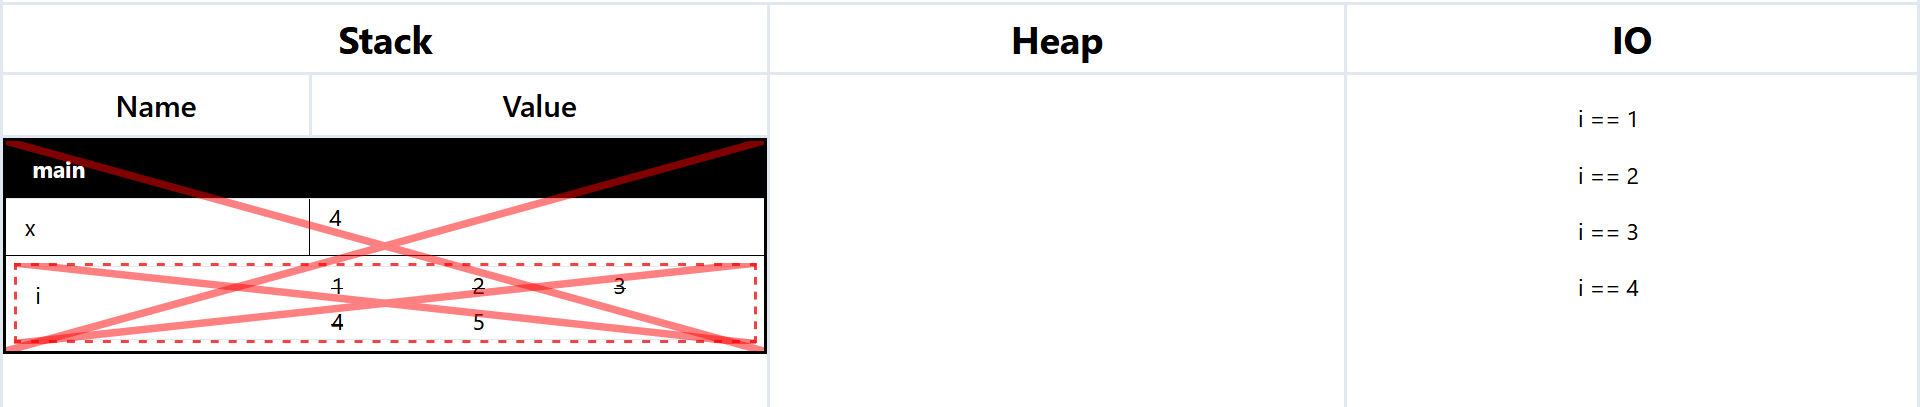
\includegraphics{forBasic.png}
\end{figure}

\subsection{Scoped Variable}

\begin{verbatim}
	public static void main (String[] args) {
	    int x = 4;
	    for (int i = 1; i < 5; i++) {
	        int temp = i + 2;
	    }
	}
\end{verbatim}

\begin{itemize}
	\item scoped variables within the loop are crossed out after the loop completes
\end{itemize}

\begin{figure}[H]
	\centering
	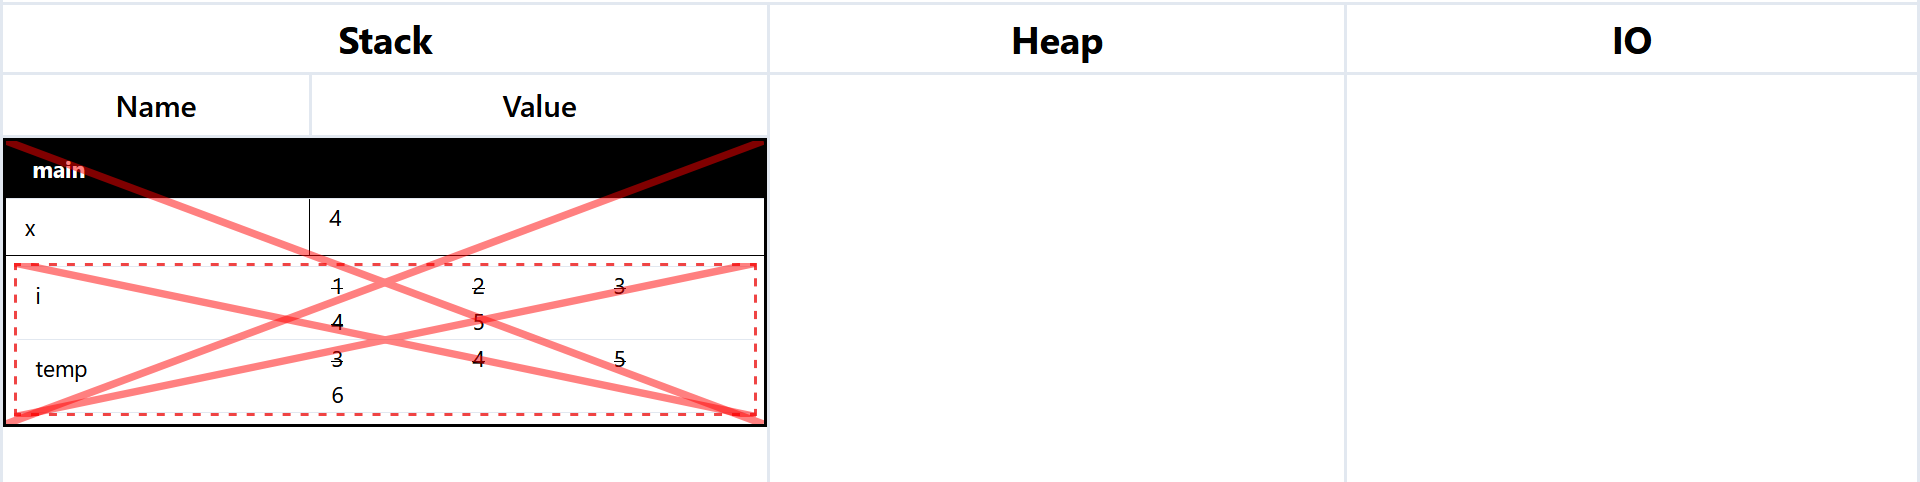
\includegraphics{forScoped.png}
\end{figure}

\pagebreak


\section{ArrayLists}

\begin{verbatim}
	public static void main (String[] args) {
	    ArrayList<Integer> arr1 = new ArrayList<>();
	    for (int x = 0; x < 4; x++) {
	        arr1.add(x);
	    }
	    System.out.println(arr1);
	    ArrayList<Integer> arr2 = arr1;
	    System.out.println(arr2);
	}
\end{verbatim}

\begin{itemize}
	\item note that the assignment statement for arr2 assigns the memory address
	and does not do a deep copy
	\begin{itemize}
		\item this point is emphasized for newer programmers
	\end{itemize}
	\item memory addresses all start with 0x to indicate that they are
	hexadecimal numbers.
	\begin{itemize}
		\item heap addresses are typically given 3 digit numbers
		\item numbers are typically written in decimal as it is easier for
		students to grasp at first (as they are not familiar with hexadecimal,
		this detail will be corrected in later courses)
		\item numbers are randomly generated and just must agree on the stack and heap
	\end{itemize}
\end{itemize}

\begin{figure}[H]
	\centering
	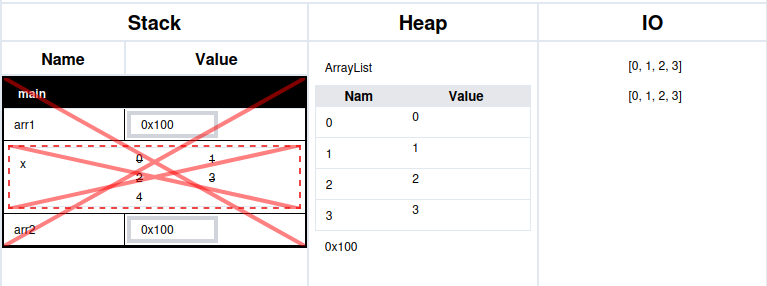
\includegraphics{arrayLists.png}
\end{figure}

\pagebreak

\subsection{Passed to functions}

\begin{verbatim}
	public static int sum(ArrayList<Integer> arrIn) {
	    int out = 0;
	    for (int x = 0; x < arrIn.size(); x++) {
	        out += arrIn.get(x);
	    }
	    return out;
	}

	public static void main (String[] args) {
	    ArrayList<Integer> arr1 = new ArrayList<>();
	    for (int x = 0; x < 4; x++) {
	        arr1.add(x);
	    }
	    System.out.println(arr1);
	    ArrayList<Integer> arr2 = arr1;
	    System.out.println(arr2);
	    int total = sum(arr1);
	    System.out.println("total: " + total);
	}
\end{verbatim}

\begin{itemize}
	\item when passing variables to functions as arguments the value on the
	stack associated with the variable name is the argument to the function
	that sets the parameter
	\item the dashed lines around index indicate that it is a scoped variable
	that only exists while the loop exists
\end{itemize}

\begin{figure}[H]
	\centering
	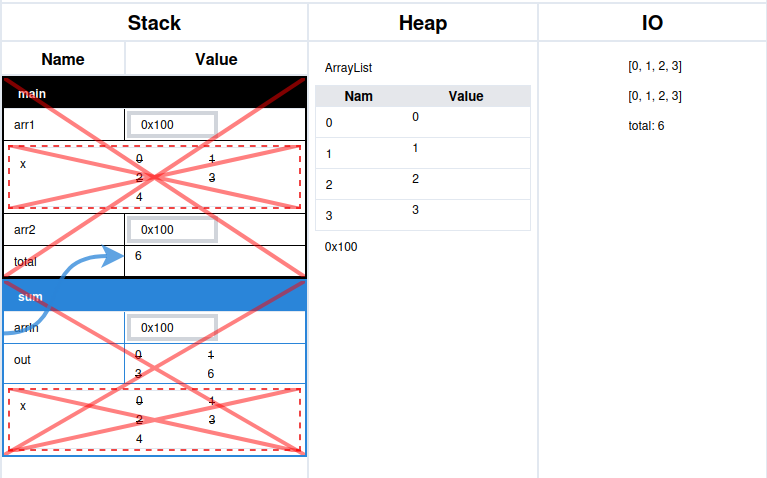
\includegraphics{arrayListsFunc.png}
\end{figure}

\pagebreak


\section{HashMaps}

\begin{verbatim}
	public static void main (String[] args) {
	    HashMap<String, Integer> bills = new HashMap<>();
	    
	    bills.put("Allen", 17);
	    bills.put("Diggs", 14);
	    
	    for (String keys: bills.keySet()) {
	      System.out.println(keys);
	    }
	}
\end{verbatim}

\begin{itemize}
	\item HashMaps are like dictionaries in python
	\item we loop through them in a manner more similar to loops in python
	\item note that the loop still has scoped variables like the previous for loop
\end{itemize}

\begin{figure}[H]
	\centering
	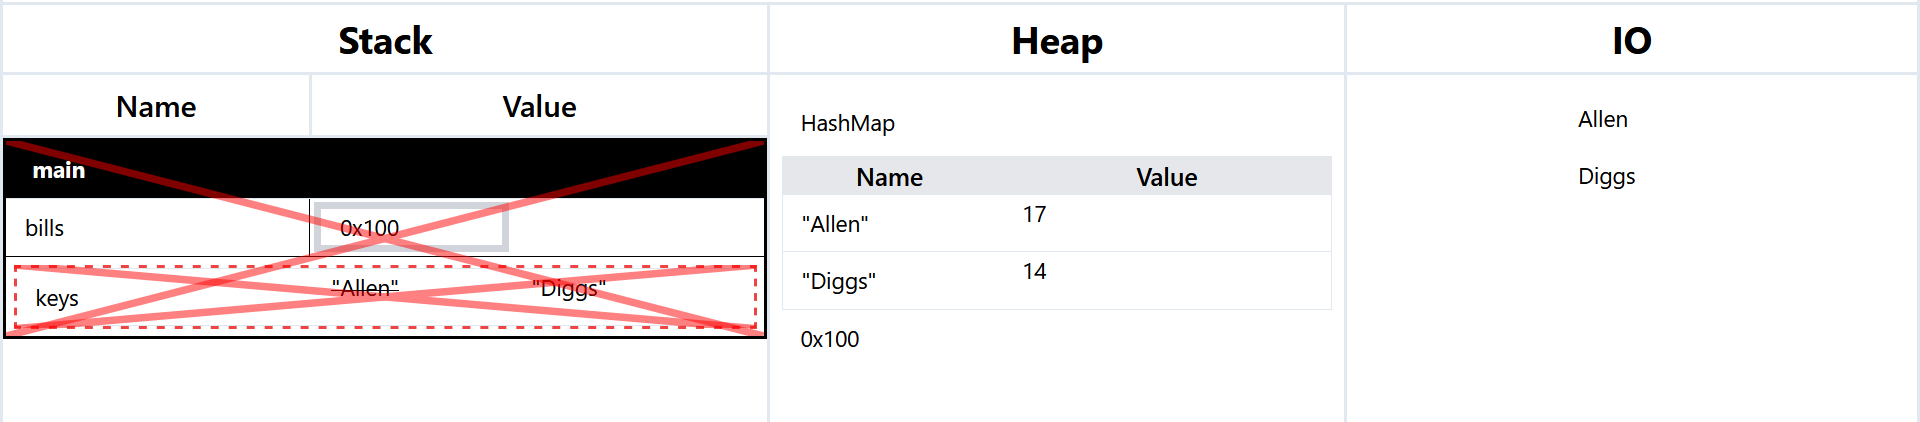
\includegraphics{hashMaps.png}
\end{figure}

\pagebreak


\section{Recursion}

\subsection{Standard Recursion}

\begin{verbatim}
	public static int computeGeometricSum(int n) {
	    if (n > 0) {
	        int result = computeGeometricSum(n - 1);
	        result += n;
	        return result;
	    } else {
	        return 0;
	    }
	}

	public static void main (String[] args) {
	    int result = computeGeometricSum(3);
	}
\end{verbatim}

\begin{itemize}
	\item each new call of cGS is performed in a new color
	\begin{itemize}
		\item returned values are kept in the color of the method that returns it
	\end{itemize}
\end{itemize}

\begin{figure}[H]
	\centering
	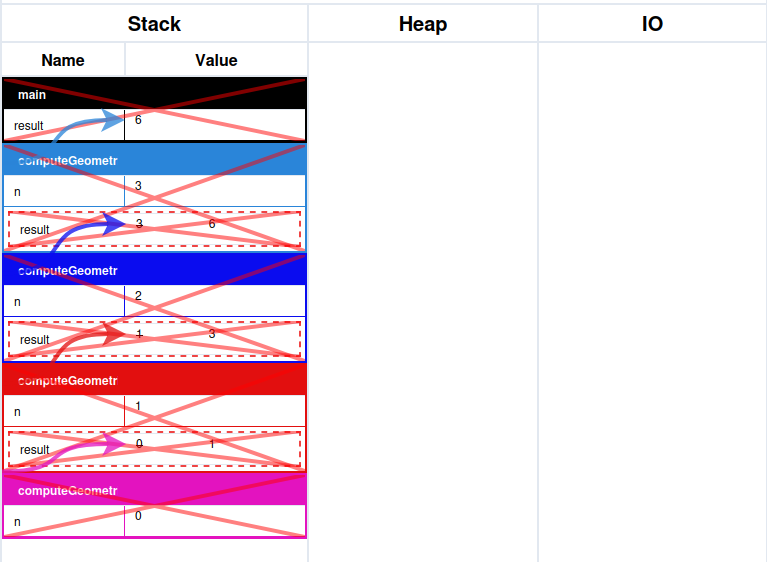
\includegraphics{recursionStandard.png}
\end{figure}

\pagebreak

\subsection{Tail Recursion}

\begin{verbatim}
	public static int computeGeometricSumTail(int n, int total) {
	    if (n > 0) {
	        return computeGeometricSum(n - 1, total + n);
	    } else {
	        return total;
	    }
	}

	public static int cGSTHelper(int n) {
	    return computeGeometricSumTail(n, 0);
	}

	public static void main (String[] args) {
	    int result = cGSTHelper(3);
	}
\end{verbatim}

\begin{itemize}
	\item each new call of cGST is performed in a new color
	\begin{itemize}
		\item returned values are kept in the color of the method that returns it
	\end{itemize}
	\item Note that the returns go to the previous function's return and not a variable
	\begin{itemize}
		\item this is why the memory of a stack frame can be released before
		the following recursive function call finishes
	\end{itemize}
\end{itemize}

\begin{figure}[H]
	\centering
	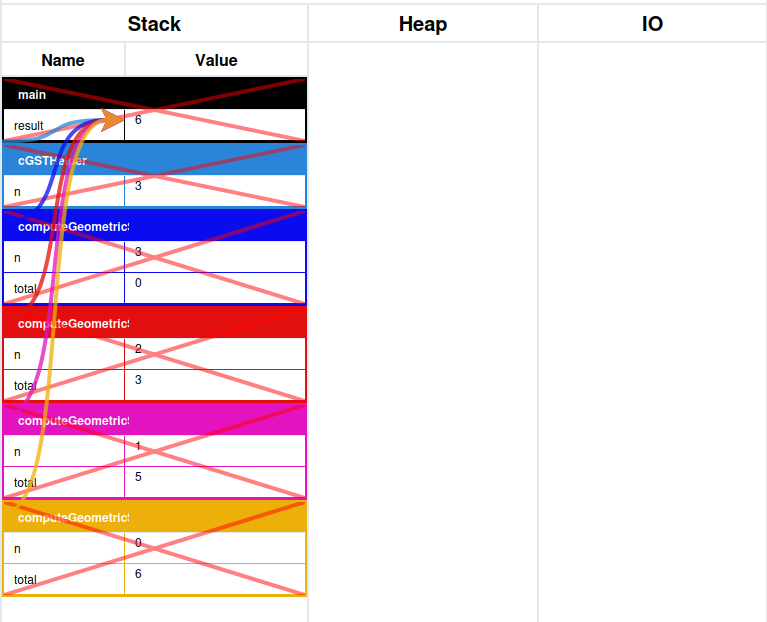
\includegraphics{recursionTail.png}
\end{figure}

\pagebreak


\section{Classes}

\begin{verbatim}
public class Player {
    private double xLoc;
    private double yLoc;
    private int maxHP;
    private int HP;
    private int damageDealt;

    public Player(double xLoc, double yLoc, int maxHP) {
        this.xLoc = xLoc;
        this.yLoc = yLoc;
        this.maxHP = maxHP;
        this.HP = maxHP;
        this.damageDealt = 4;
    }
    public int getHP() {
        return this.HP;
    }
    public void takeDamage(int damage) {
        this.HP -= damage;
    }
    public void attack(Player otherPlayer) {
        otherPlayer.takeDamage(this.damageDealt);
    }
    public void move(double dx, double dy) {
        this.xLoc += dx;
        this.yLoc += dy;
    }

    public static void main(String[] args) {
        Player player1 = new Player(0.0, 0.0, 10);
        Player player2 = new Player(7.0, -4.0, 10);
        player2.move(-6.5, 3.4);
        player2.attack(player1);
    }
}
\end{verbatim}

\begin{figure}[H]
	\centering
	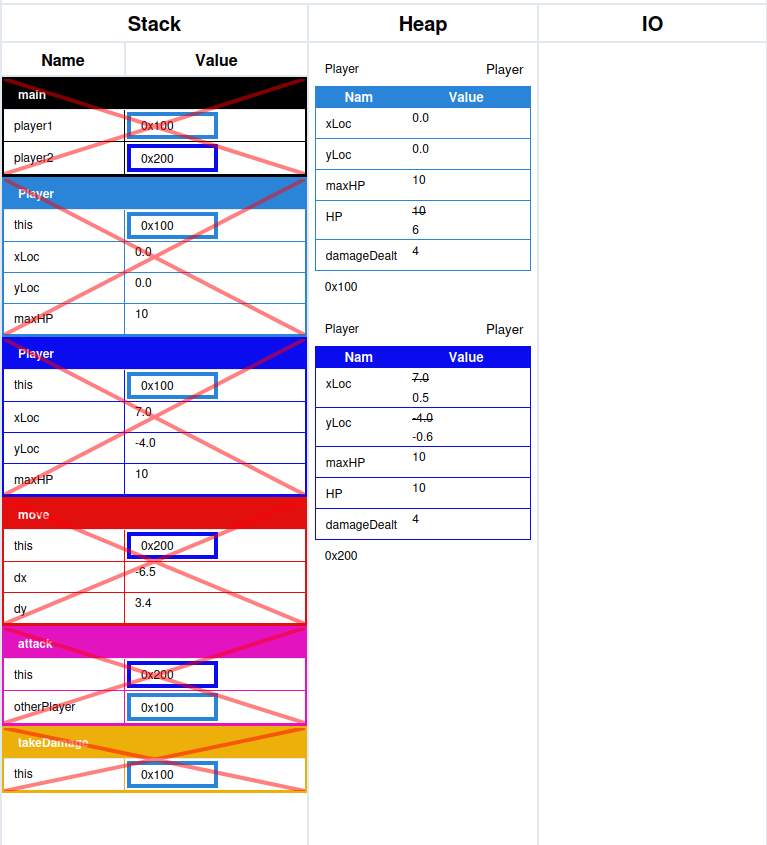
\includegraphics{classes.png}
\end{figure}

\pagebreak


\section{Inheritance}

\begin{verbatim}
public class GameItem {
    private double xLoc;
    private double yLoc;

    public GameItem(double xLoc, double yLoc) {
        this.xLoc = xLoc;
        this.yLoc = yLoc;
    }
    public void move(double dx, double dy) {
        this.xLoc += dx;
        this.yLoc += dy;
    }
}

public class Teleporter extends GameItem {
    private double dx;
    private double dy;

    public Teleporter(double xLoc, double yLoc, double dx, double dy) {
        super(xLoc, yLoc);
        this.dx = dx;
        this.dy = dy;
    }

    public static void main(String[] args) {
        Teleporter t = new Teleporter(2, 2, 3, 3);
        t.move(2, 3);
    }
}
\end{verbatim}

\begin{figure}[H]
	\centering
	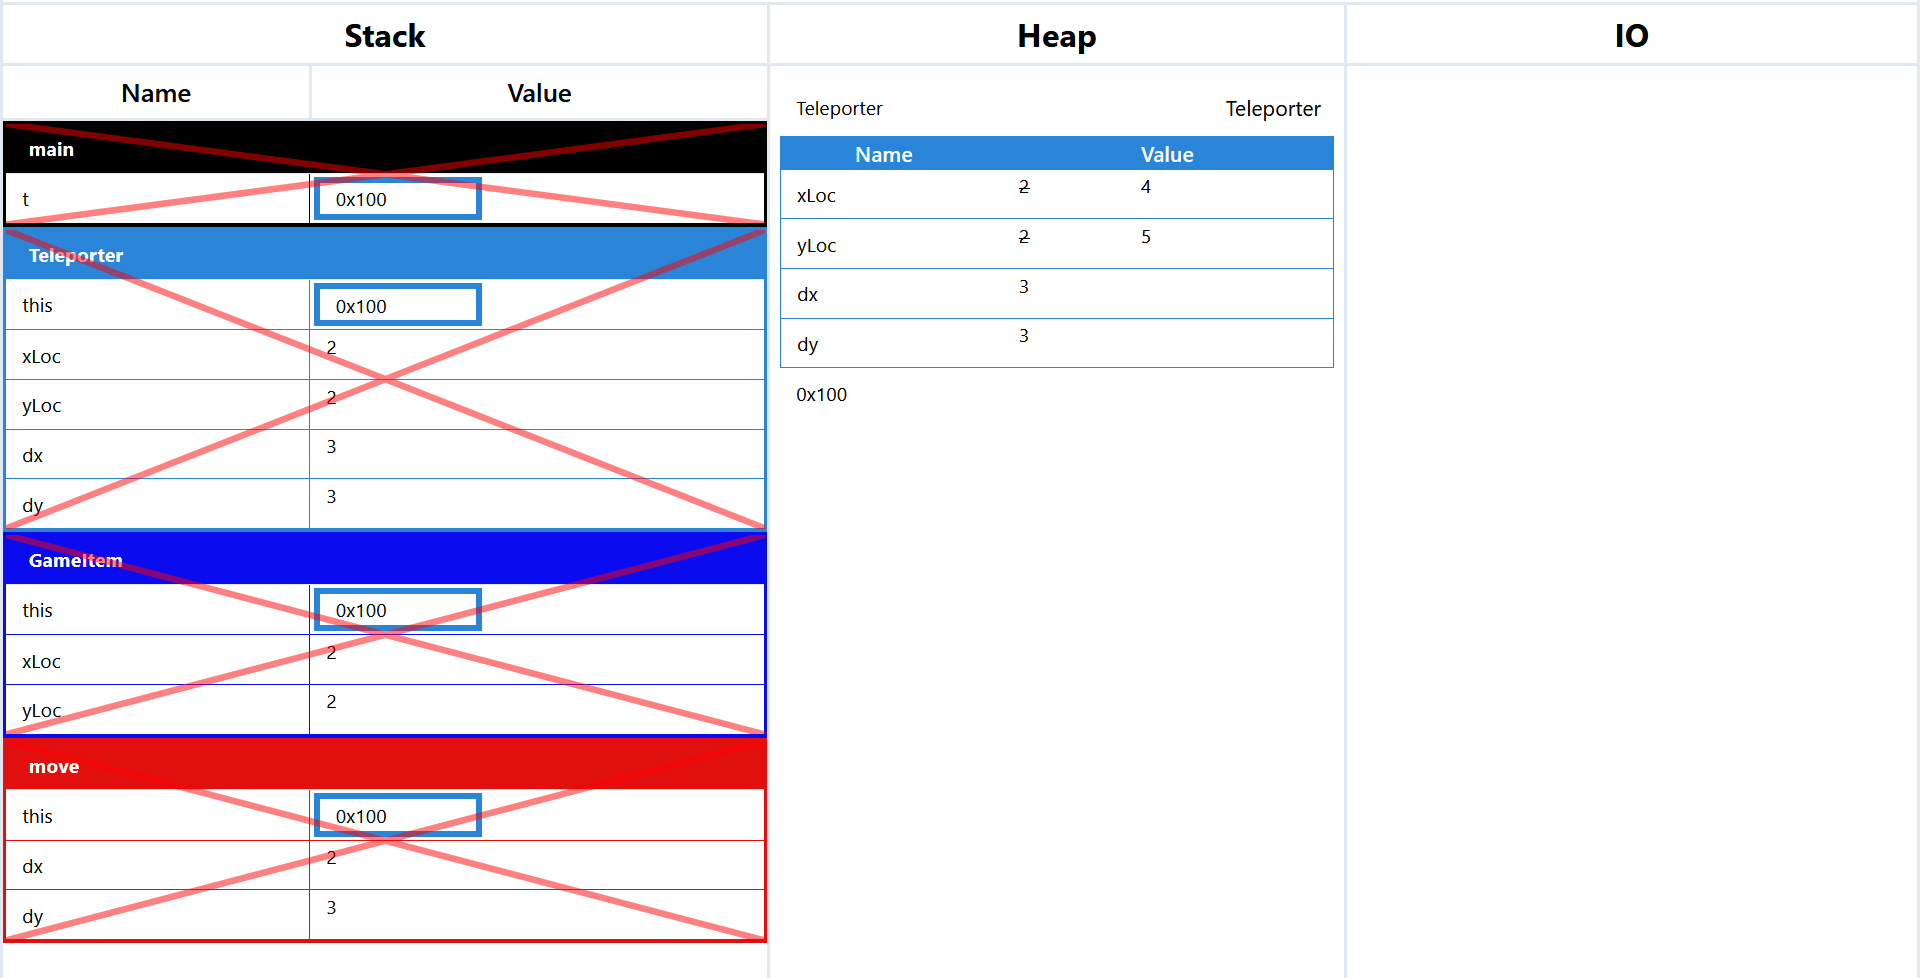
\includegraphics{inheritance.png}
\end{figure}

\pagebreak


\section{Polymorphism}

\begin{verbatim}
public class A {
    protected int a;

    public A(int a) {
        this.a = a;
    }
}

public class B extends A{
    private int b;

    public B(int b) {
        super(b);
        this.b = b*2;
    }
}

public class C extends A{
    private int c;

    public C(int a, int c) {
        super(a);
        this.c = c;
    }
}

public class RunABC {
    public static void main(String[] args) {
        A a = new A(1);
        A b = new B(2);
        A c = new C(3, 4);
    }
}
\end{verbatim}

\begin{figure}[H]
	\centering
	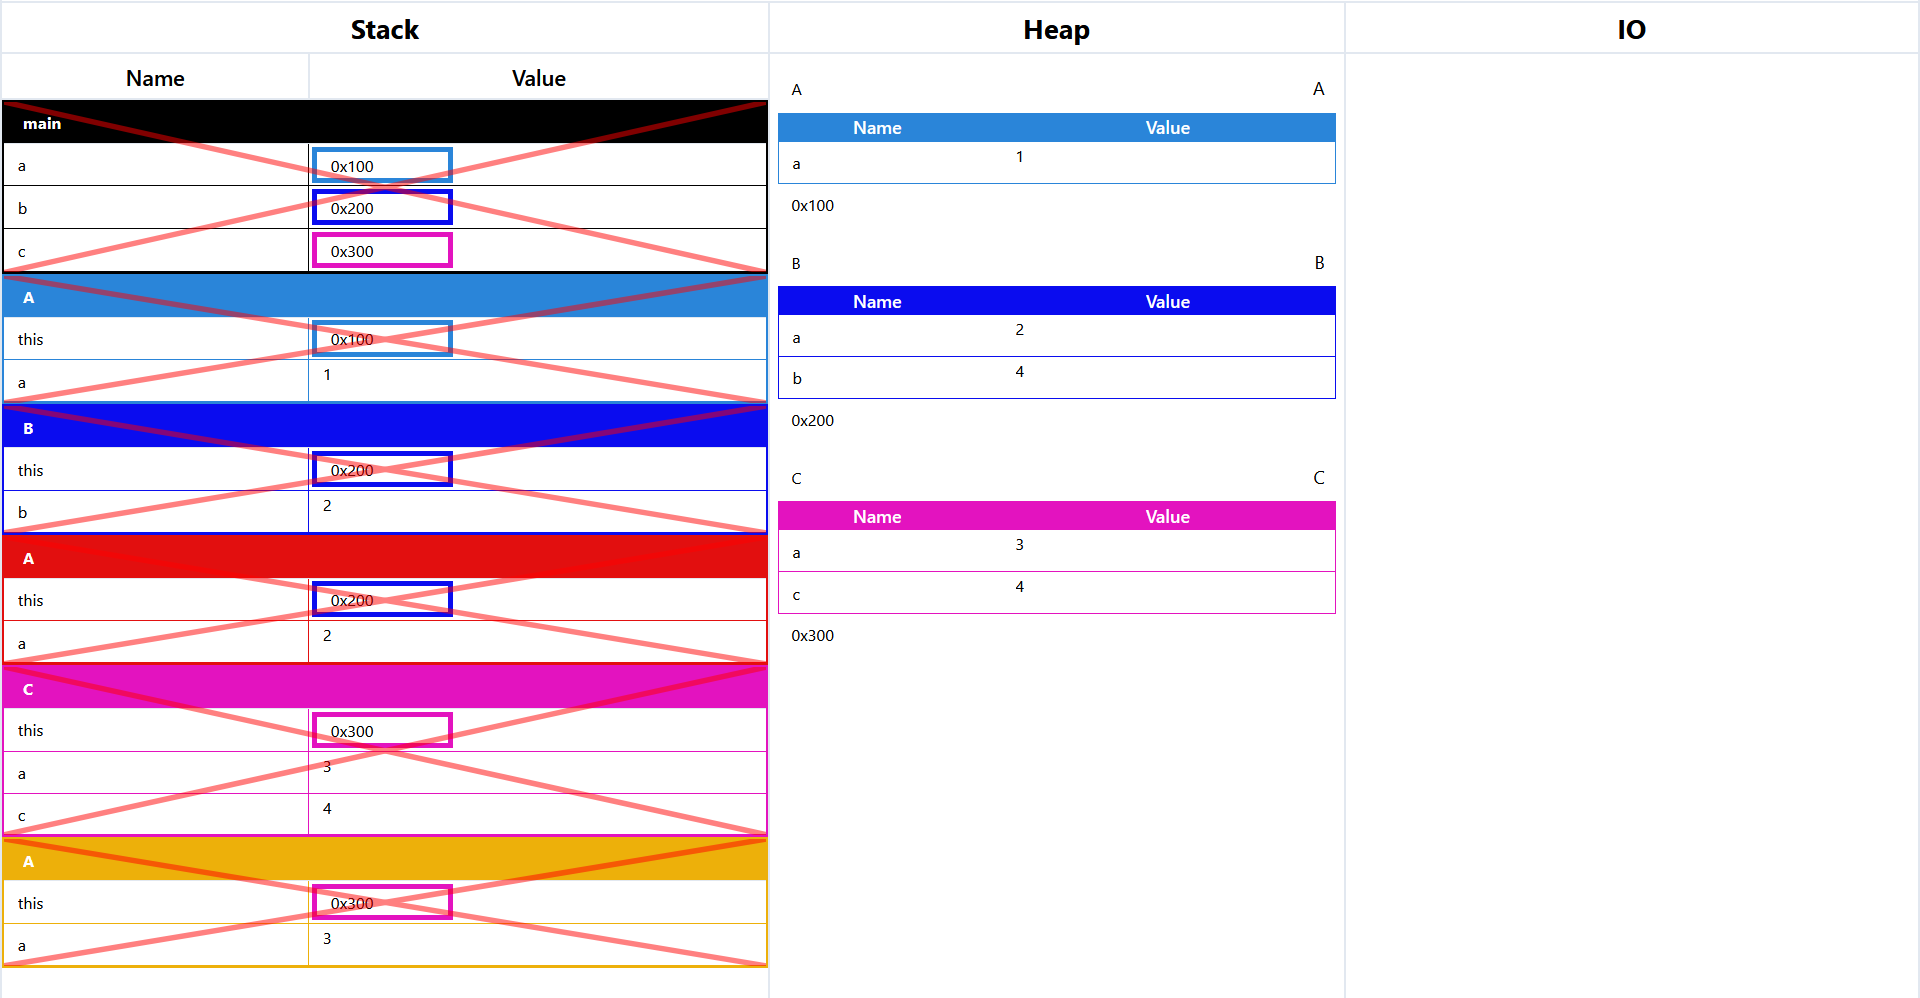
\includegraphics{polymorphism.png}
\end{figure}

\end{document}
